\documentclass{article}

\usepackage[utf8]{inputenc}
\usepackage{tikz}
\usepackage{tkz-euclide}
\usepackage{enumitem}

\begin{document}
\section*{Geometry Drawing in \LaTeX}

Drawing geometry in~\LaTeX~is~supported through various methods ranging from~native environments to~specialized packages. The built-in \texttt{picture} environment allows for~the placement of~basic shapes such~as \texttt{\textbackslash line}, \texttt{\textbackslash circle}, and~\texttt{\textbackslash vector} by~specifying coordinates with~the \texttt{\textbackslash put} command. While~efficient for~simple diagrams, more~complex scientific illustrations typically utilize the \texttt{TikZ} package, which provides a~powerful framework for~defining paths and~nodes with~mathematical precision.



Choose a~numbered entry point to~begin the~learning process:

\begin{enumerate} \item \textbf{Native Foundations}: Exploring the~basic \texttt{picture} environment and~coordinate-based positioning using \texttt{\textbackslash put} and~\texttt{\textbackslash qbezier}. \item \textbf{The TikZ Framework}: An~introduction to~modern vector graphics, focusing on~flexible path commands and~logical node structures. \item \textbf{Classical Euclidean Geometry}: Utilizing \texttt{tkz-euclide} to~create precise geometric constructions like angle bisectors, circles, and~intersections. \end{enumerate}

\begin{tikzpicture}
    \tkzDefPoint(0,0){A}
    \tkzDefPoint(5,2){B}

    \tkzDrawSegment(A,B)

    \tkzDrawPoints(A,B)
\end{tikzpicture}
\begin{tikzpicture}
  % 1. Define points
  \tkzDefPoint(0,0){A}
  \tkzDefPoint(5,0){B}
  \tkzDefPoint(2,4){C}

  % 2. Define the Incircle (calculates center and radius point)
  \tkzDefInCircle(A,B,C) 
  
  % 3. Get the center point and name it 'I'
  \tkzGetPoint{I}

  \tkzDefPointBy[projection=onto A--B](I)

  \tkzGetPoint{perm}

  \tkzDrawPoints(I,perm)

  \tkzAutoLabelPoints[center=I](A,B,C,I)
  \tkzLabelPoint(perm){T}
  % 4. Draw the triangle and the circle
  \tkzDrawPolygon(A,B,C)
  \tkzDrawCircle[color=blue](I,perm) % Note: this syntax varies slightly
\end{tikzpicture} \\
\begin{tikzpicture}[]
  % 1. Define the Triangle Vertices
  \tkzDefPoint(0,0){A}
  \tkzDefPoint(5,0){B}
  \tkzDefPoint(2,4){C}
  \tkzDrawPolygon(A,B,C)

  % 2. "Define" the Bisector Lines
  % We find a second point on the bisector of angle A and angle B
  \tkzDefBisectorLine(B,A,C) \tkzGetPoint{a}
  \tkzDefBisectorLine(A,B,C) \tkzGetPoint{b}

  % 3. "Use" the lines to find the intersection (The Incenter)
  \tkzInterLL(A,a)(B,b) \tkzGetPoint{I}
  
  % 4. "Define" the radius by projecting I onto the line (A,B)
  \tkzDefPointBy[projection=onto A--B](I) \tkzGetPoint{H}

  % 5. Draw the results
  \tkzDrawCircle(I,H)
  \tkzDrawPoints(A,B,C,I,H)
  \tkzLabelPoints[below](A,B,I,H)
  \tkzLabelPoints[above](C)
\end{tikzpicture}
\begin{tikzpicture}[scale=1]
  % 1. Define the three points
  \tkzDefPoint(0,0){A}
  \tkzDefPoint(5,1){B}
  \tkzDefPoint(2,4){C}
  
  % 2. Define the perpendicular bisector of AB
  % 'mediator' is the term for perpendicular bisector in tkz-euclide
  \tkzDefLine[mediator](A,B) \tkzGetPoints{m1}{m2}
  
  % 3. Define the perpendicular bisector of BC
  \tkzDefLine[mediator](B,C) \tkzGetPoints{n1}{n2}
  
  % 4. Find the intersection of the two bisectors (The Center)
  \tkzInterLL(m1,m2)(n1,n2) \tkzGetPoint{O}
  
  % 5. Drawing
  \tkzDrawPolygon(A,B,C)           % Draw the triangle
  \tkzDrawLines[dashed, blue](m1,m2 n1,n2) % Draw the bisector lines
  \tkzDrawCircle(O,A)              % Draw the circle (Center O, through A)
  
  % 6. Labeling
  \tkzDrawPoints(A,B,C,O)
  \tkzLabelPoints[below](A,B)
  \tkzLabelPoints[above](C,O)
\end{tikzpicture}
\begin{tikzpicture}[scale=1.2]
  % 1. Define and Draw the Triangle Points
  \tkzDefPoint(0,0){A}
  \tkzDefPoint(5,0.5){B}
  \tkzDefPoint(1.5,4){C}
  \tkzDrawPolygon(A,B,C)
  
  % --- STEP 1: BISECTING LINE AB ---
  
  % A. Calculate the intersection points (The math behind the scenes)
  % This finds the two points where the "compass arcs" would cross.
  \tkzDefLine[mediator](A,B) \tkzGetPoints{mAB1}{mAB2}
  
  % B. Draw the "Compass Arcs"
  % We tell LaTeX: "Draw a compass mark from A to that intersection point"
  \tkzCompass[color=red, delta=20](A,mAB1)
  \tkzCompass[color=red, delta=20](B,mAB1)
  
  \tkzCompass[color=red, delta=20](A,mAB2)
  \tkzCompass[color=red, delta=20](B,mAB2)
  
  % C. Draw the bisector line passing through those marks
  \tkzDrawLine[color=red, dashed](mAB1,mAB2)
  
  
  % --- STEP 2: BISECTING LINE BC ---
  
  % A. Calculate intersection points
  \tkzDefLine[mediator](B,C) \tkzGetPoints{mBC1}{mBC2}
  
  % B. Draw the "Compass Arcs"
  \tkzCompass[color=blue, delta=20](B,mBC1)
  \tkzCompass[color=blue, delta=20](C,mBC1)
  
  \tkzCompass[color=blue, delta=20](B,mBC2)
  \tkzCompass[color=blue, delta=20](C,mBC2)
  
  % C. Draw the bisector line
  \tkzDrawLine[color=blue, dashed](mBC1,mBC2)
  
  
  % --- STEP 3: THE RESULT ---
  
  % Find the intersection of the two red and blue lines
  \tkzInterLL(mAB1,mAB2)(mBC1,mBC2) \tkzGetPoint{O}
  
  % Draw the final Circumcircle
  \tkzDrawPoint[color=black](O)
  \tkzLabelPoint[below](O){$O$}
  \tkzDrawCircle(O,A)
  
  \tkzAutoLabelPoints[center=O](A,B,C)
\end{tikzpicture}
\begin{tikzpicture}[scale=1]
  \tkzDefPoint(0,0){A}
  \tkzDefPoint(5,0){B}
  \tkzDrawSegment(A,B)
  \tkzLabelPoints(A,B)

  % 1. Find the intersection points (same as before)
  % We use a fixed radius (3.5cm)
  \tkzInterCC[R](A,3.5cm)(B,3.5cm) \tkzGetPoints{C}{D}

  % 2. Draw compass arcs ONLY for the top point (C)
  % We skip drawing arcs for D!
  \tkzCompass[color=red, delta=20](A,C)
  \tkzCompass[color=red, delta=20](B,C)

  % 3. Find the midpoint of A and B
  \tkzDefMidPoint(A,B) \tkzGetPoint{M}
  
  % 4. Draw the bisector
  % Connect the top intersection (C) through the midpoint (M)
  % We extend the line a bit past M using the 'add' option
  \tkzDrawLine[add=0 and 0.5, color=blue, dashed](C,M)
  
  % Optional: Mark the right angle
  \tkzMarkRightAngle[german](B,M,C)

\end{tikzpicture}
\newpage
\begin{tikzpicture}
\tkzDefPoint(0,0){O}
\tkzDefPoint(0,2){r}
\tkzDefPoints{5/0/P}

\tkzDrawSegment[color=blue](O,P)

\tkzDefLine[mediator](O,P) \tkzGetPoints{md1}{md2}

\tkzCompasss(P,md1 P,md2 O,md1 O,md2)
\tkzDrawSegment[dashed,color=blue](md1,md2)

\tkzInterLL(O,P)(md1,md2) \tkzGetPoint{S}

\tkzDrawCircle[color=blue](S,P)

\tkzInterCC(S,P)(O,r) \tkzGetPoints{T1}{T2}

\tkzDrawLines[thick](P,T1 P,T2)

\tkzDrawCircle(O,r)
\tkzDrawPoints(O,P)
\tkzLabelPoints(O,P,T1,T2)
\end{tikzpicture} \\
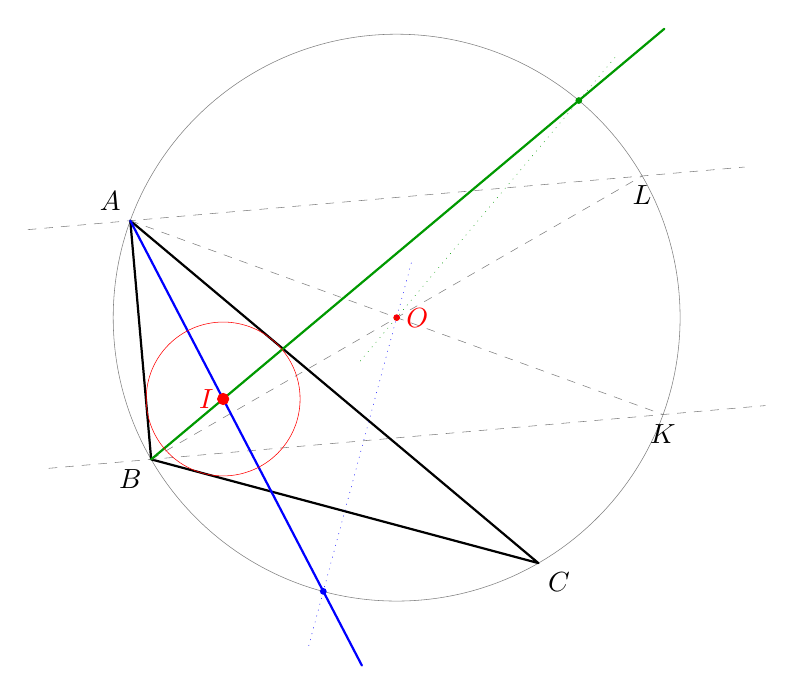
\begin{tikzpicture}[scale=1.2]
  % --- ZADÁNÍ ---
  % Definujeme kružnici a tři body (skrytý střed O pro výpočty)
  \tkzDefPoint(0,0){O}
  \tkzDefPoint(3,0){R} % Poloměr pro definici
  \tkzDefPoint(160:3){A}
  \tkzDefPoint(210:3){B}
  \tkzDefPoint(300:3){C}
  
  % Vykreslíme zadání (Kružnice a trojúhelník)
  \tkzDrawCircle(O,R)
  \tkzDrawPolygon[thick](A,B,C)
  \tkzLabelPoints[above left](A)
  \tkzLabelPoints[below left](B)
  \tkzLabelPoints[below right](C)

  % --- KROK 1: HLEDÁNÍ STŘEDU O (Thaletova věta) ---
  
  % Kolmice k AB v bodě B -> Průměr K
  \tkzDefLine[orthogonal=through B](A,B) \tkzGetPoint{dir1}
  \tkzInterLC(B,dir1)(O,A) \tkzGetPoints{}{K}
  \tkzDrawLine[dashed, color=gray](B,K)
  \tkzDrawSegment[dashed, color=gray](A,K) % Toto je průměr

  \tkzLabelPoints(K)
  
  % Kolmice k AB v bodě A -> Průměr L
  \tkzDefLine[orthogonal=through A](A,B) \tkzGetPoint{dir2}
  \tkzInterLC(A,dir2)(O,A) \tkzGetPoints{L}{}
  \tkzDrawLine[dashed, color=gray](A,L)
  \tkzDrawSegment[dashed, color=gray](B,L) % Toto je průměr

  \tkzLabelPoints(L)
  
  % Kolmice k AC v bodě C -> Průměr L
%   \tkzDefLine[orthogonal=through C](A,C) \tkzGetPoint{dir2}
%   \tkzInterLC(C,dir2)(O,A) \tkzGetPoints{}{L}
%   \tkzDrawLine[dashed, color=gray](C,L)
%   \tkzDrawSegment[dashed, color=gray](A,L) % Toto je průměr

%   \tkzLabelPoints(L)
  
  % (V kódu už máme O definované, ale geometricky je to průsečík AK a CL)
  % Vykreslíme nalezený střed O
  \tkzDrawPoint[color=red](O)
  \tkzLabelPoint[right, color=red](O){$O$}


  % --- KROK 2: OSY ÚHLŮ POMOCÍ STŘEDŮ OBLOUKŮ ---
  
  % A) Osa úhlu alfa (při A)
  % Vedeme kolmici ze středu O na stranu BC.
  % Tato kolmice protne kružnici v půlícím bodě oblouku (S_a).
  \tkzDefLine[orthogonal=through O](B,C) \tkzGetPoint{dirBC}
  \tkzInterLC(O,dirBC)(O,A) \tkzGetPoints{S_a}{S_a_far} 
  % S_a je ten bod na opačné straně než A
  
  \tkzDrawLine[dotted, color=blue](O,S_a)
  \tkzDrawPoint[color=blue](S_a)
  \tkzDrawLine[add=0 and 0.2, color=blue, thick](A,S_a) % Osa úhlu


  % B) Osa úhlu beta (při B)
  % Vedeme kolmici ze středu O na stranu AC.
  \tkzDefLine[orthogonal=through O](A,C) \tkzGetPoint{dirAC}
  \tkzInterLC(O,dirAC)(O,A) \tkzGetPoints{S_b_far}{S_b}
  
  \tkzDrawLine[dotted, color=green!60!black](O,S_b)
  \tkzDrawPoint[color=green!60!black](S_b)
  \tkzDrawLine[add=0 and 0.2, color=green!60!black, thick](B,S_b) % Osa úhlu


  % --- VÝSLEDEK ---
  % Průsečík os
  \tkzInterLL(A,S_a)(B,S_b) \tkzGetPoint{I}
  \tkzDrawPoint[color=red, size=4](I)
  \tkzLabelPoint[left, color=red](I){$I$}
  
  % (Volitelné) Vykreslení vepsané kružnice pro kontrolu
  \tkzDefPointBy[projection=onto A--B](I) \tkzGetPoint{Touch}
  \tkzDrawCircle[color=red](I,Touch)

\end{tikzpicture}
\end{document}